To complete most of home serving tasks, our robot consists of three major parts: chassis based on Mecanum wheel, UR5 arm including Robotiq-G85 hand. Tinker is about 140cm in height. 
\subsubsection{Chassis}
Tinker can move in any direction easily owing to the Mecanum chassis. The chassis consists of 4 separated Mecanum wheel systems, each of which consists of a Mecanum wheel, a DJI M3058P19 motor. The PC sends control message to the stm32 to command the chassis to move as planed based on ROS. The chassis has a size of $800\text{mm} \times 500\text{mm}\times 200\text{mm}$.
\begin{figure}[!t]
\centering
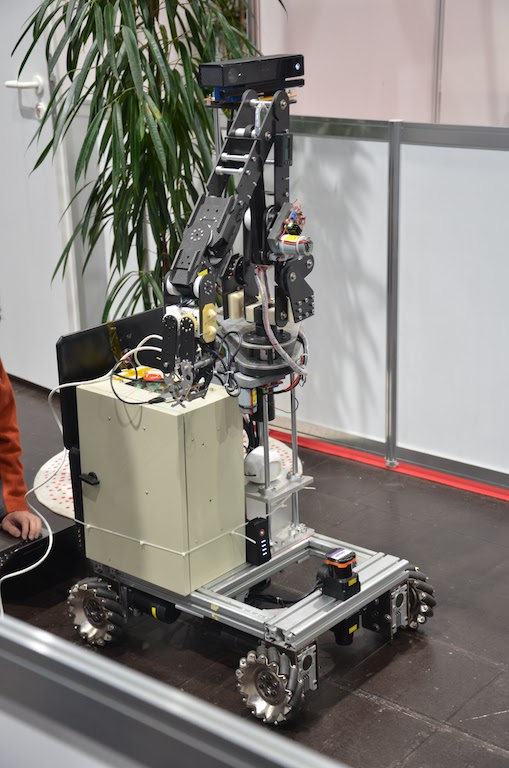
\includegraphics[scale=0.2]{tinker.jpg}
    \caption{Picture of tinker robot}
\end{figure}

\subsubsection{Robot arm and hand}
The robot arm and hand are the most major part of the mobile robot, used to grasp objects.UR5 is long and powerful enough to hold most of the objects at home, and Robotiq-G85 gives a reliable grasping.A laser transmitter and receiver sensor is used to confirm the grasping.
\begin{figure*}[!t]
	\centering
    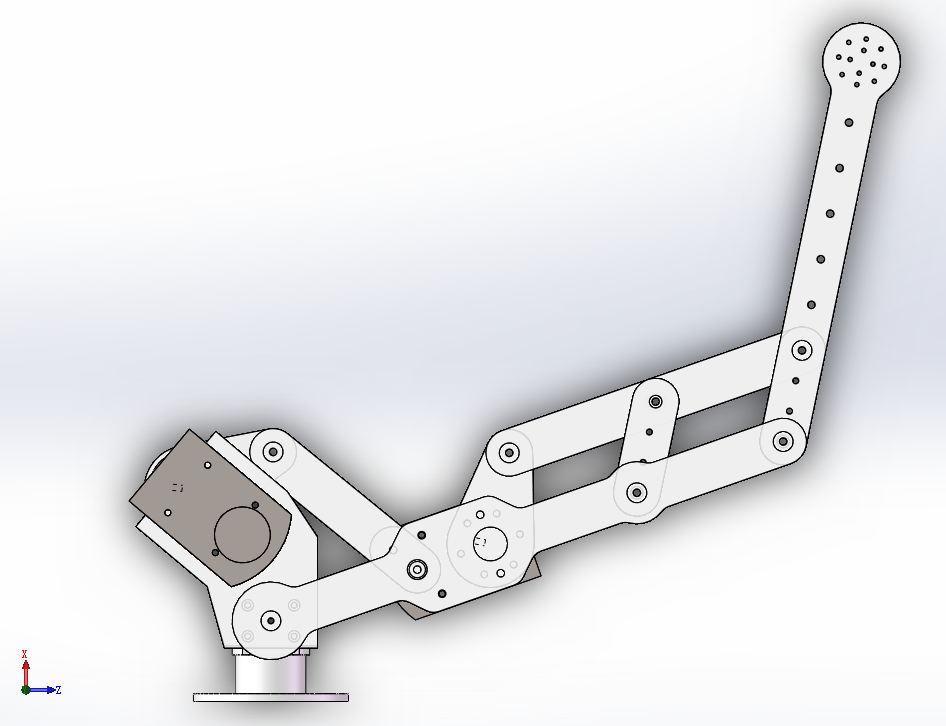
\includegraphics[scale=0.2]{arm.jpg}
    \caption{Robotic Arm and Hand}
\end{figure*}

